\chapter{Software Evaluation}
\label{chap:data_collection}

In dieser Semesterarbeit wurde zwar keine ausf{\"u}hrliche Software Evaluation vorgenommen, da dies nicht Teil der Zielsetzung war. Dennoch wurde rudiment{\"a}r m{\"o}gliche Software betrachtet und die Vor- und Nachteile jeweils abgewogen und anschliessend eine Auswahl getroffen. Im Folgenden sind die Software Komponenten, deren Vor- und Nachteile sowie die Entscheidungen dokumentiert.

\section{Container}
\label{sec:container}

Ein Container ist ein Gef{\"a}ss, welches es erm{\"o}glicht Anwendungen auf unterschiedlichen Plattformen ohne grossen Aufwand einzusetzen und zu verteilen. Ein Anwendung, welche mit einem oder mehreren Containern realisiert wird, l{\"a}uft sowohl auf Linux-, Windows oder macOS, also weitgehend unabh{\"a}ngig vom Betriebssystem der Infrastruktur. Das Container-Image beinhaltet alles, was zum Ausf{\"u}hren der Anwendung erforderlich ist: Code, Laufzeit- und Systemtools, Systembibliotheken und Einstellungen.

Container-Images werden zur Laufzeit zu sogenannten Containern. Im Falle von Docker, werden Container-Images 'Docker Images' genannt, dieser werden bei Aufruf zu 'Docker Containern'. Gesteuert wird dies durch die sogenannte,  Docker Engine (oder einen Docker compatiblen container daemon). Container isolieren einerseits die Software von ihrer Umgebung und stellen andererseits sicher, dass sie trotz Unterschieden in der verwendeten Infrastruktur, z.B. zwischen Entwicklung und Staging, einheitlich funktioniert.

\textbf{Entscheidung}

F{\"u}r den ersten Durchstich, welcher lokal auf dem Notebook mit macOS laufen soll wird Docker verwendet, da Docker bereits lokal auf den Macbook installiert ist und dadurch kein zus{\"a}tzlicher Aufwand f{\"u}r Installation und Konfiguration entsteht. Der Einsatz von 'docker-compose' erlaubt es zudem, mehrere Docker Container gleichzeitig zu starten und untereinander kommunizieren zu lassen.

Um die Streaming und Analyseumgebung auf dem \href{http://bigboards.io/orderprototype/}{BigBoards nHex} (Big Data Cluster) zu betreiben wird Kubernetes anstatt Docker Swarm verwendet. Kubernetes hat eine gr{\"o}ssere Verbreitung in produktiven Umgebungen und somit ein gr{\"o}sseres Angebot an Tutorials. Ebenfalls wird Kubernetes von allen grossen Cloud Anbietern unterst{\"u}tzt, falls ein on-prem Einsatz nicht praktikabel sein sollte. Da f{\"u}r beide Varianten, Kubernetes resp. docker-swarm eine Einarbeitung meinerseits n{\"o}tig ist, wurde die Entscheidung entsprechend der gr{\"o}sseren Community und Cloud Provider Support gef{\"a}llt.

Eine kurze Gegen{\"u}berstellung von Docker Swarm und Kubernetes ist in Abbildung \ref{fig:kub_vs_dokcer} ersichtlich. Die ausf{\"u}hrliche Beschreibung zu der Grafik ist auf dem Blog  \href{https://dev.to/totalcloudio/docker-swarm-vs-kubernetes--what-you-really-need-to-know--4kjb}{dev.to} zu finden.

\begin{figure}[H]
	\centering
		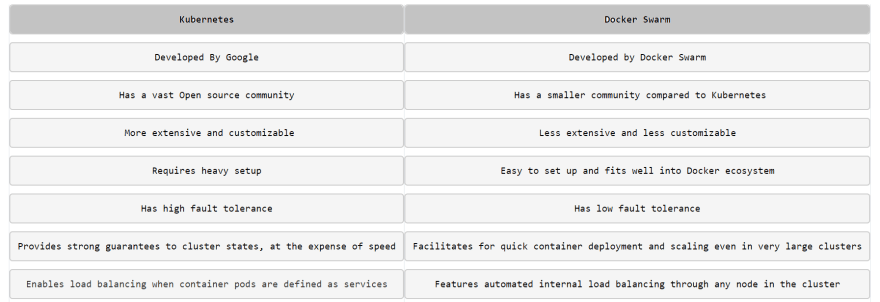
\includegraphics[scale=0.5 ]{images/docker_kubernetes.png}
	\caption{Kubernetes vs Docker Swarm}

	\label{fig:kub_vs_dokcer}
\end{figure}

\subsection{Docker}
\label{sec:Docker}
 \href{https://www.docker.com}{Docker} ist eine kostenlose Open Source Software, welche Containervritualisierung anbietet und basiert auf Linux Technologien. Urspr{\"u}nglich ist Docker auf die Virualisierung mit Linux ausgerichtet, kann jedoch auch auf Windows und macOS verwendet werden. Docker f{\"u}hrt die Container auf einer einzigen Maschine aus. 

Um mehrere Container, die eine logische Anwendung ergeben, zu managen wird \href{https://docs.docker.com/compose/}{docker-compose} verwendet. Es wird eine sogenannte Compose-Datei erstellt, welche die verwendeten docker images und deren Software Tools und Konfigurationen enth{\"a}lt. Jeder Eintrag in diesem File stellt sp{\"a}ter einen einzelnen Container da. Der Vorteil liegt darin, dass es nur eine einzige Datei ben{\"o}tigt wird um:

\begin{itemize}
  \item Container zu definieren und konfigurieren
  \item Die Kommunikation zwischen Containern sicherzustellen
  \item Container zu starten
  \item Container zu stoppen
\end{itemize}
 
Docker eignet sich jedoch prim{\"a}r f{\"u}r den Einsatz auf einem Computer/Server. Um die Anwendung auf einem Cluster mit mehreren Nodes (Servern) betreiben zu k{\"o}nnen muss \href{https://docs.docker.com/engine/swarm/}{ Docker Swarm} verwendet werden. Docker Swarm ist ein Orchestrierungs- und Clustering-Tool, welches die Sammlung von Containern (und die Kommunikation zwischen ihnen) {\"u}ber ein Netzwerk organisiert.

\subsection{Kubernetes}
\label{sec:Kubernetes}
\href{https://kubernetes.io}{Kubernetes} ist, {\"a}hnlich wie Docker Swarn, eine kostenlose Open Source Software, welche die Orchestrierung von Containern erm{\"o}glicht und wurde urspr{\"u}nglich von Google als Plattform f{\"u}r automatische Deployments, Skalierung und Betrieb ihrer Software entwickelt. Ein grundlegender Unterschied zwischen Kubernetes und anderen bedeutenden Orchestrierungswerkzeugen besteht in der Art der Virtualisierungsumgebungen, die sie verwalten k{\"o}nnen. W{\"a}hrend Docker Swarm Mode als natives Docker-Orchestrierungstool eben diese Containerumgebung voraussetzt, unterst{\"u}tzt Kubernetes auch andere containerbasierte Virtualisierungssysteme, sogar als heterogene Umgebungen. Apache DCOS kontrolliert und steuert dar{\"u}ber hinaus auch nicht containerisierte Rechenressourcen\footnote{\label{foot:2} \url{https://www.dev-insider.de/was-ist-kubernetes-a-633462/}}.


\section{ETL/ELT und Streaming-Software}
\label{sec:streaming}

ETL/ELT (extract transform load / extract load transform) Tools wurden entwickelt, um den Datenfluss zwischen unterschiedlichen Softwarekomponenten und Datenbanken zu automatisieren und dabei erste Datenverarbeitungen automatisiert vorzunehmen:

\begin{itemize}
  \item Extraktion der relevanten Daten aus unterschiedlichen Quellen
  \item Transformation der Daten in die ben{\"o}tigte Form
  \item Speichern (load) der Daten in die Zieldatenbank
  \item Je nach Einsatzbereich und Zweck k{\"o}nnen dabei die Schritte Transform und Load ihre Positionen tauschen.
\end{itemize}

Der beschriebene Vorgang ist Batch orientiert und l{\"a}uft - bedingt durch eine lange Laufzeit grosser Batches - meistens Nachts. Somit skaliert es schlecht und eignet sich nur bedingt f{\"u}r Anwendungen im Big Data Bereich. Als Folge dessen wurden die klassischen ETL/ELT Tools weiter entwickelt und es entstanden Streaming Anwendungen, welche mit schnellen Datenlieferungen und grossen Datenmengen in Echtzeit umgehen k{\"o}nnen.

\subsection{Apache NiFi}

\href{https://nifi.apache.org}{Apache NiFi} ist ein Open-Source-Projekt, entwickelt von der Apache Software Foundation. Es basiert auf dem Konzept der Datenflussprogrammierung, was bedeutet, dass dieses ETL-Tool es erm{\"o}glicht, Piplienes visuell zusammenzustellen: Dadurch wird der Einsatz ohne Programmierkenntnisse erm{\"o}glicht. NiFi kann mit verschieden Quellen arbeiten: Zum Beispiel RabbitMQ, JDBC-Abfrage, Hadoop, MQTT, UDP-Socket, etc. Um die Daten zu prozessieren bietet das Tool M{\"o}glichkeiten um die Daten zu filtern, anzupassen, zu verbinden, aufzuteilen, zu erweitern und zu {\"u}berpr{\"u}fen. 

Vorteile: 
\begin{itemize}
  \item Perfekte Umsetzung des Konzepts der Datenflussprogrammierung
  \item M{\"o}glichkeit, bin{\"a}re Daten zu verarbeiten
  \item Datenherkunft
\end{itemize}

Nachteile: 
\begin{itemize}
  \item Vereinfachte Benutzeroberfl{\"a}che 
  \item Fehlende Live-{\"U}berwachung und Statistiken pro Datensatz
\end{itemize}

\subsection{StreamSets}

\href{https://streamsets.com}{StreamSets} wurde von einem ehemaligen Cloudera Engineering Leiter und einem ehemaligen Informatica Produkt Leiter initiiert und mit weiteren Entwicklern als Open-Source-Projekt aufgesetzt. Es besteht aus zwei komplement{\"a}ren Produkten - StreamSets Data Collector (alias SDC) und StreamSets Dataflow Performance Manager (alias DPM).

Vorteile: 
\begin{itemize}
  \item Jeder Prozessor hat individuelle Statistiken pro Datensatz mit sch{\"o}ner Visualisierung f{\"u}r effektives Debugging. 
  \item Attraktive Benutzeroberfl{\"a}che
  \item Gutes ETL/ELT-Tool f{\"u}r Streaming oder dateibasierte Daten
\end{itemize}

Nachteile: 
\begin{itemize}
  \item Fehlende wiederverwendbare JDBC-Konfiguration 
  \item Die {\"A}nderung einer Einstellung eines Prozessors erfordert das Stoppen des gesamten Datenflusses der betroffenen Pipeline.
\end{itemize}
 

\subsection{Airflow}

\href{https://airflow.apache.org}{Airflow} ist eine Plattform f{\"u}r die Gestaltung, Erstellung und Verfolgung von einzelnen Workflows. Sie kann mit Cloud Services wie GCP, Azure und AWS verwendet werden und es besteht die M{\"o}glichkeit, Airflow auf Kubernetes mit Astronomer Enterprise zu betreiben. Die Workflows sind in Python geschrieben, aber die Schritte selbst k{\"o}nnen beliebig ausgef{\"u}hrt werden. Airflow wurde als flexibler Task Scheduler entwickelt. 

Vorteile: 
\begin{itemize}
  \item Geeignet f{\"u}r verschiedene Arten von Aufgaben
  \item Benutzerfreundliche Oberfl{\"a}che f{\"u}r eine {\"u}bersichtliche Visualisierung
  \item Skalierbare L{\"o}sung
\end{itemize}

Nachteile: 
\begin{itemize}
  \item Ist nicht geeignet f{\"u}r Streaming-Auftr{\"a}ge 
  \item Erfordert zus{\"a}tzliche Operatoren
\end{itemize}

\subsection{Tool Entscheid}
F{\"u}r die Semesterarbeit wird StreamSets eingesetzt. Airflow wurde ausgeschlossen, weil es sich f{\"u}r Streaming nicht eignet. NiFi kam aus pers{\"o}nlichen Gr{\"u}nden f{\"u}r mich nicht infrage, da es urspr{\"u}nglich von der NAS entwickelt und eingesetzt wurde. 2014 wurde  NiFi als open source zur Verf{\"u}gung gestellt.

\section{Messaging: Kafka}
\label{sec:messaging}

\href{http://kafka.apache.org}{Apache Kafka} ist eine Open-Source-Plattform f{\"u}r Streaming, die es erm{\"o}glicht, Daten mit hohem Durchsatz und geringer Latenzzeit zu {\"u}bertragen. Kafka wurde urspr{\"u}nglich bei LinkedIn konzipiert und 2011 Open-Source entwickelt und hat seitdem eine breite Akzeptanz in der Community gefunden. Mittlerweile ist es das bevorzugte Echtzeit-Messaging-System in der Branche. Ein sogenannter Kafka Producer schreibt (ver{\"o}ffentlicht) Nachrichten und ein Kafka Consumer liest (abonniert) diese. Weitere Informationen zu Kafka und dessen Funktionen sind der Projektseite zu entnehmen\footnote{\label{foot:3} \url{https://kafka.apache.org/intro}}.


\section{Datenbanken}
\label{sec:datenbanken}

Die Entscheidung f{\"u}r MongoDB und Elasticsearch wurde ganz am Anfang der Semesterarbeit gef{\"a}llt. F{\"u}r die Datenspeicherung der Rohdaten von Twitter fiel die Entscheidung auf MongoDB, da diese sehr einfach aufzusetzen ist und die Rohdaten ohne Transformation direkt in ihrem JSON Format persistiert werden k{\"o}nnen. MongoDB kann auch ohne Probleme mit Anpassungen an der Datenstruktur umgehen und speichert das neue Dokument.

Elasticsearch wurde gew{\"a}hlt, da es Textdaten sind, welche in einem JSON Format vorliegen und Elasticsearch in Verbindung mit Kibana (ELK stack) eine perfekte Erg{\"a}nzung f{\"u}r Volltextsuche und Analyse ist. 

\subsection{MongoDB}
\href{https://www.mongodb.com}{MongoDB} ist eine NoSQL Open-Source-Datenbank, die ein dokumentenorientiertes Datenmodell verwendet. Die Architektur von MongoDB beruht auf Sammlungen (Collections) und Dokumenten und  unterst{\"u}tzt das dynamische Schema-Design. Dies bedeutet, dass die Dokumente in einer Collection verschiedene Felder und Strukturen haben k{\"o}nnen.

\subsection{Elasticsearch}
\href{https://www.elastic.co/products/elastic-stack}{Elasticsearch} ist eine Suchmaschine auf Basis von Lucene. Das in Java geschriebene Programm speichert Dokumente in einem NoSQL-Format (JSON) und die Kommunikation mit Klienten erfolgt {\"u}ber ein RESTful-Webinterface. Elasticsearch ist neben Solr die am weitesten verbreitete Search-Engine. Elasticsearch erm{\"o}glicht auf einfache Weise den Betrieb im Rechnerverbund zur Umsetzung von Hochverf{\"u}gbarkeit und Lastverteilung. \footnote{\label{foot:4} \url{https://www.heise.de/developer/artikel/Volltextsuche-mit-ElasticSearch-1920454.html}}


\section{Dashboard}
\label{sec:dashboard}
\subsection{Kibana}
\href{https://www.elastic.co/products/elastic-stack}{Kibana} ist eine browserbasierte Open-Source-Analyseplattform, welche auf der Elasticsearch Engine aufbaut\footnote{\label{foot:5} \url{https://github.com/elastic/kibana}}. Sie erm{\"o}glicht die Suche und Visualisierung der in Elasticsearch-Indizes enthaltenen Daten\footnote{\label{foot:6} \url{https://www.heise.de/developer/meldung/Kibana-4-mit-neuem-Visualisierungsframework-ausgestattet-2555851.html}}. 

Da Elasticsearch verwendet wird, wird Kibana f{\"u}r die Visualisierung des Dashbaords genutzt. Andere Tools, wie z.B. Grafana, wurden aus diesem Grund nicht weiter betrachtet.

\section{Zusammenfassung der Entscheidungen}
\label{sec:zusammenfassung}

Zusammengefasst, siehe Abbildung \ref{fig:used_sw}, werden folgende Software Komponenten f{\"u}r diese Semesterarbeit verwendet:
\begin{itemize}
  \item Container: Docker (lokal mit mit docker-compose)
  \item Orchestrierung im Cluser: Kubernetes
  \item Streaming-Software: StreamSets
  \item Datenbanken: MongoDB, Elasticsearch
  \item Visualisierung \& Analyse: Kibana
  \item APIs: Twitter, Here (f{\"u}r die Aufl{\"o}sung von Geokoordinaten in Twitter-Feeds)
\end{itemize}

\begin{figure}[H]
	\centering
		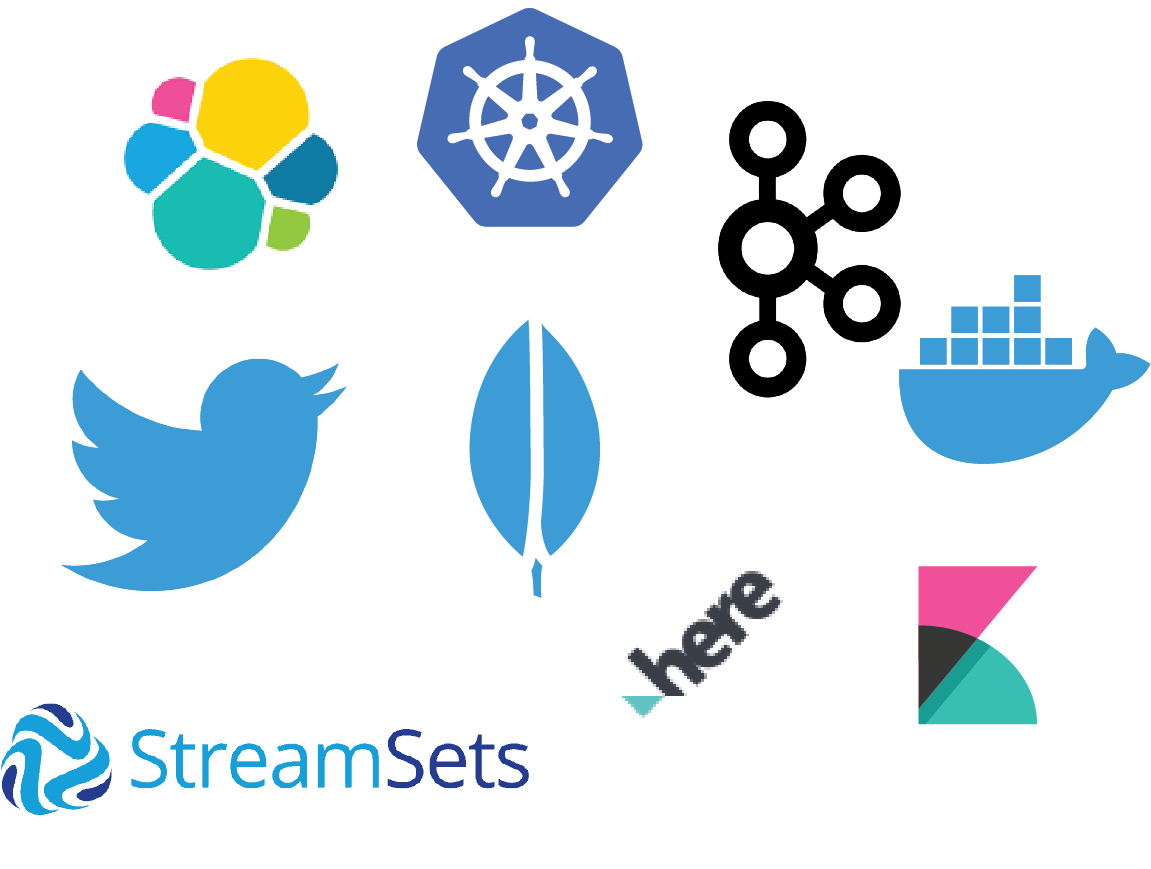
\includegraphics[scale=0.8 ]{images/used_sw.png}
	\caption{Eingesetzte Software}
	\label{fig:used_sw}
\end{figure}




